\documentclass[aspectratio=169]{ctexbeamer} %[t]:顶端对齐
\usepackage{ctex}
\usepackage{listings}
\usepackage{xcolor}
\usepackage{tikz}
\usetikzlibrary{intersections,through}
\usetikzlibrary{arrows.meta,calc}
\usepackage{pgfplots}
\pgfplotsset{compat=1.18} %兼容到1.18版及以下版本的特性
\usepackage{amssymb,amsmath}
\usepackage{enumitem}
\usepackage{setspace} %设置行间距
%\usepackage{geometry}
%\usetheme{Madrid} %Madrid,蓝色调为主。
%\usecolortheme{beaver} %beaver
%\usefonttheme{professionalfonts}


\date{\today}
\begin{document}

\begin{frame}[fragile]
\frametitle{LaTex文档结构}

\unilstset{TeX}
\begin{lstlisting}
\documentclass{...} % ... 为某文档类
% 导言区
\begin{document}
% 正文内容
\end{document}
% 此后内容会被忽略
\end{lstlisting}

\end{frame}

\begin{frame}[fragile]
\frametitle{LaTex作图模板代码}

\unilstset{TeX}
\begin{lstlisting}
\documentclass [tikz, border=12pt] {standalone}

\begin{document}

\begin{tikzpicture}

%详细作图的指令

\end{tikzpicture}

\end{document}
\end{lstlisting}

\end{frame}

\begin{frame}[fragile]
\frametitle{LaTex作图-画线}

\lstset{
  language=TeX,
  basicstyle=\ttfamily\small,
  backgroundcolor=\color{lightgray},
  keywordstyle=\color{orange},
  commentstyle=\color{red},
  stringstyle=\color{blue},
  frame=single, 
  numbers=left,
  label={lst:sum},
}
\begin{lstlisting}
\documentclass [tikz, border=12pt] {standalone}

\begin{document}
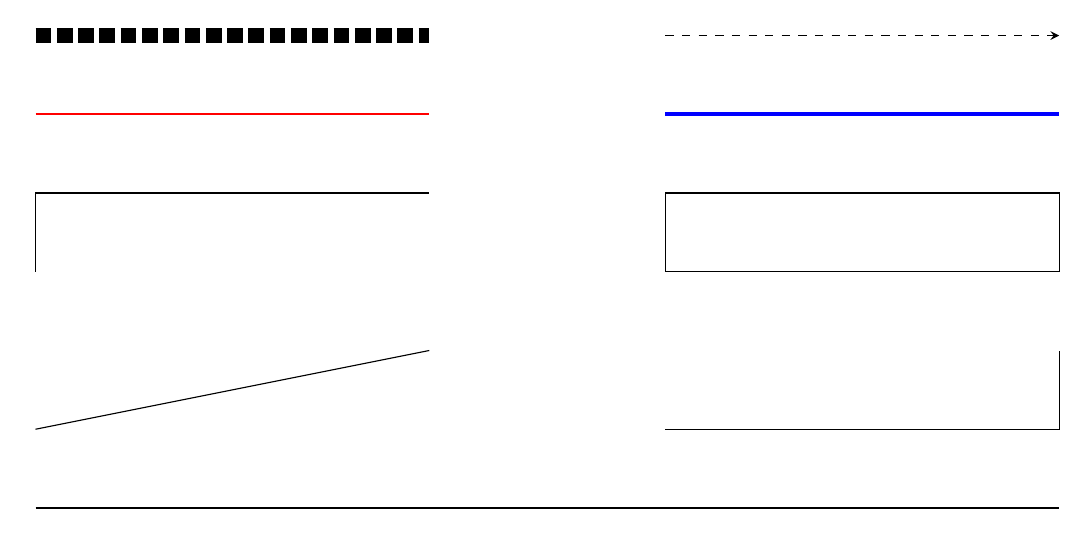
\begin{tikzpicture}

\draw (1,0)  -- (14,0); % 画一条线
\draw (1,1) to (6,2); % 画一条线
\draw (9,1) -| (14,2); % 画一条折线(先水平,后垂直)
\draw (1,3) |- (6,4) ; % 画一条折线(先垂直,后水平)
\draw (9,3) rectangle (14,4); % 画一个矩形
\draw [red,thick] (1,5) -- (6,5); % 红色,粗细:thick
\draw [blue,ultra thick] (9,5) -- (14,5); % 蓝色,ultra thick
\draw [dotted,line width=0.2cm] (1,6) -- (6,6); % 点线,线宽0.2cm
\draw [dashed,->,>=stealth] (9,6) -- (14,6) ; % 虚线,stealth箭头

\end{tikzpicture}
\end{document}
\end{lstlisting}
\end{frame}
\begin{frame}[fragile]
\frametitle{LaTex作图-等边三角形1}

\unilstset{TeX}
\begin{lstlisting}
\documentclass[tikz, border=12pt]{standalone}
\usetikzlibrary{intersections, through}
\begin{document}
\begin{tikzpicture}
    \coordinate (A) at (0, 0); % 定义坐标A
    \coordinate (B) at (5, 0); % 定义坐标B
    \draw[thick, dashed, name path=CA] (A) circle (5); % 绘制圆CA
    \draw[thick, dashed, name path=CB] (B) circle (5); % 绘制圆CB
    \path [name intersections={of=CA and CB, by={P}}]; % 求交点P
    \filldraw[black] (P) circle (1pt); % 给点P画上实心圆
    \draw[thick] (A) -- (P) -- (B) -- cycle; % 绘制等边三角形
    \node[below left] at (A) {A}; % 标注A
    \node[below right] at (B) {B}; % 标注B
    \node[above] at (P) {P}; % 标注P
\end{tikzpicture}
\end{document}
\end{lstlisting}
\end{frame}

\begin{frame}[fragile]
\frametitle{LaTex作图-等边三角形2}

\lstset{
  language=TeX,
  basicstyle=\ttfamily\small,
  backgroundcolor=\color{lightgray},
  keywordstyle=\color{orange},
  commentstyle=\color{red},
  stringstyle=\color{blue},
  frame=single, 
  numbers=left,
  label={lst:sum},
}
\begin{lstlisting}
\documentclass[tikz, border=12pt]{standalone}
\usepackage{tikz}
\usetikzlibrary{intersections}
\begin{document}
\begin{tikzpicture}

\coordinate (A) at (0, 0); % 定义点A
\coordinate (B) at (5, 0); % 定义点B
\draw[name path=A1] (A)+(55:5) arc(55:65:5); % 画圆弧A1,A为圆心,55-65度,半径5
\draw[name path=A2] (B)+(125:5) arc(125:115:5); % 画圆弧A2,B为圆心,125-115度,半径5
\path [name intersections={of=A1 and A2, by=P}]; % 求交点P
\draw[thick] (A) -- (B) -- (P) -- cycle; % 画连接A, B, P的三角形
\node at (A) [below left] {A}; % 标注点A
\node at (B) [below right] {B}; % 标注点B
\node at (P) [above] {P}; % 标注点P

\end{tikzpicture}
\end{document}

\end{lstlisting}
\end{frame}

\begin{frame}[fragile]
\frametitle{LaTex作图-等边三角形3}

\lstset{
  language=TeX,
  basicstyle=\ttfamily\small,
  backgroundcolor=\color{lightgray},
  keywordstyle=\color{orange},
  commentstyle=\color{red},
  stringstyle=\color{blue},
  frame=single, 
  numbers=left,
  label={lst:sum},
}
\begin{lstlisting}
\documentclass[tikz, border=10pt]{standalone}
\usetikzlibrary{intersections,through}
\begin{document}
\begin{tikzpicture}
    % 定义点 A、B、C的坐标
    \coordinate (A) at (0:0);
    \coordinate (B) at (0:5);
    \coordinate (C) at (60:5);
    
    % 标注点A、B、C
    \node[below left] at (A) {$A$};
    \node[below right] at (B) {$B$};
    \node[above] at (C) {$C$};
    
    % 绘制从 A 到 B 的线段
    \draw[thick] (A) -- (B) -- (C) -- (A);
\end{tikzpicture}
\end{document}
\end{lstlisting}
\end{frame}

\begin{frame}[fragile]
\frametitle{LaTex作图-等边三角形4}

\lstset{
  language=TeX,
  basicstyle=\ttfamily\small,
  backgroundcolor=\color{lightgray},
  keywordstyle=\color{orange},
  commentstyle=\color{red},
  stringstyle=\color{blue},
  frame=single, 
  numbers=left,
  label={lst:sum},
}
\begin{lstlisting}
\documentclass[tikz, border=10pt]{standalone}
\usetikzlibrary{intersections,through}
\begin{document}
\begin{tikzpicture}
    % 定义点 A 和 B
    \coordinate (A) at (0,0);
    \coordinate (B) at (5,0);
    
    % 绘制原始线段 AB
    \draw[thick] (A) --++ (60:5) coordinate (C) -- (B) -- cycle;
    \node at (A) [below left] {$A$};
    \node at (B) [below right] {$B$};
    \node at (C) [above] {$C$}; 
\end{tikzpicture}
\end{document}
\end{lstlisting}
\end{frame}


\end{document}